\chapter{Generative Adversarial Networks (GANs)}
\label{ch:gan}

At the heart of unsupervised learning lies the ambition to model the underlying probability distribution of observed data. Given a dataset $\mathcal{D} = \{x_1, \dots, x_N\}$ drawn independent and identically distributed from an unknown, high-dimensional distribution $P_{\text{data}}$ over a space $\mathcal{X}$, the standard statistical approach involves specifying a parameterized family of distributions $p_\theta(x)$ and finding the parameters $\theta$ that maximize the likelihood of the data. This framework, known as prescribed generative modeling, is elegant and enjoys the robust statistical guarantees of maximum likelihood estimation. However, it is historically fraught with computational hurdles. Evaluating the likelihood often requires computing intractable normalizing constants (partition functions), forcing practitioners to rely on approximations like Markov Chain Monte Carlo or to impose overly restrictive structural assumptions (such as strict independence or Gaussianity) to remain tractable. 

Generative Adversarial Networks (GANs) eschew explicit density estimation entirely, offering a radical departure from classical statistics. Instead of prescribing a stochastic decoder distribution $p_\theta(x|z)$ as we did with Variational Autoencoders (see Chapter 13), GANs construct an \textit{implicit} generative model. We define a latent variable $z \in \mathcal{Z}$ with a simple, known prior distribution $p(z)$ (such as a spherical Gaussian), and a deterministic, differentiable function---typically a neural network $f_\theta$---denoted here as the generator $G_\theta : \mathcal{Z} \to \mathcal{X}$, which maps the latent noise into the data space. 

By passing the easily sampled noise $z$ through this complex, non-linear transformation, the distribution of the generated samples $x = G_\theta(z)$ induces an implicit probability measure $P_\theta$ over $\mathcal{X}$. We can easily draw samples from $P_\theta$, but we have no way to evaluate the point-wise density $p_\theta(x)$. The goal of learning is to find parameters $\theta$ such that $P_\theta$ closely approximates $P_{\text{data}}$, matching all of its higher-order moments and topological features.

Because $P_\theta$ does not provide an explicit analytical formula for the likelihood of a point $x$, we cannot directly minimize classical metrics like the Kullback-Leibler (KL) divergence via standard maximum likelihood. To bridge this gap, GANs introduce a second neural network: the \textit{discriminator} $D_\phi : \mathcal{X} \to (0, 1)$. The discriminator is a binary classifier trained to distinguish between true samples drawn from $P_{\text{data}}$ and fake samples drawn from $P_\theta$. Simultaneously, the generator $G_\theta$ is trained to fool the discriminator, updating its parameters to make its synthetic outputs indistinguishable from the real data.

This dual-network architecture fundamentally reframes density estimation as a two-player minimax game. Rather than specifying a static, pre-defined distance metric between distributions, the discriminator acts as an adaptive critic. It dynamically learns the topology of the space where $P_{\text{data}}$ and $P_\theta$ differ most, and penalizes the generator specifically along those axes. As the generator improves and its outputs become more realistic, the discriminator is forced to learn ever more subtle statistical distinctions. This escalating arms race provides a continuously updating, rich gradient signal to the generator.

The adversarial framework shifts the burden from analytical tractability to optimization over function spaces. It is a profound conceptual pivot: we substitute the calculation of an intractable integral with the optimization of an auxiliary neural network. While this trade-off allows GANs to generate astonishingly sharp, high-fidelity samples that capture the manifold structure of complex data (such as photorealistic human faces), it replaces the convex stability of maximum likelihood with the volatile dynamics of non-cooperative game theory.

In this chapter, we formalize the GAN framework. We dissect the core minimax objective, proving that under ideal nonparametric conditions, the game perfectly recovers $P_{\text{data}}$ by implicitly minimizing the Jensen-Shannon Divergence. We then rigorously examine the gradients of this game, shedding light on the catastrophic failure modes---such as vanishing gradients and mode collapse---that plague empirical GAN training when the supports of $P_{\text{data}}$ and $P_\theta$ are disjoint. This analysis sets the stage for the mathematically robust integral probability metrics and $f$-divergences explored in subsequent chapters.

\section{The Minimax Game and Implicit Distributions}

Let $\mathcal{X}$ be the data space and $\mathcal{Z}$ be the latent space. We are given a target distribution $P_{\text{data}}$ over $\mathcal{X}$ and a simple prior $p(z)$ over $\mathcal{Z}$. The generator $G_\theta: \mathcal{Z} \to \mathcal{X}$ pushes forward the measure $p(z)$ to induce a generated distribution $P_\theta$ on $\mathcal{X}$. The discriminator $D_\phi: \mathcal{X} \to (0, 1)$ outputs the probability that a sample $x$ originates from $P_{\text{data}}$ rather than $P_\theta$.

The two networks are pitted against each other in a zero-sum game defined by the value function $V(G_\theta, D_\phi)$:
\begin{equation}
    \min_\theta \max_\phi V(G_\theta, D_\phi) = \mathbb{E}_{x \sim P_{\text{data}}} [\log D_\phi(x)] + \mathbb{E}_{z \sim p(z)} [\log (1 - D_\phi(G_\theta(z)))].
\end{equation}

By the law of the unconscious statistician, we can rewrite the second expectation in terms of the induced distribution $P_\theta$:
\begin{equation}
    V(G_\theta, D_\phi) = \mathbb{E}_{x \sim P_{\text{data}}} [\log D_\phi(x)] + \mathbb{E}_{x \sim P_\theta} [\log (1 - D_\phi(x))].
\end{equation}

To understand the theoretical properties of this game, we study it in the nonparametric limit, assuming both $G_\theta$ and $D_\phi$ have infinite capacity and can represent any measurable function.

\begin{figure}[htpb]
\centering
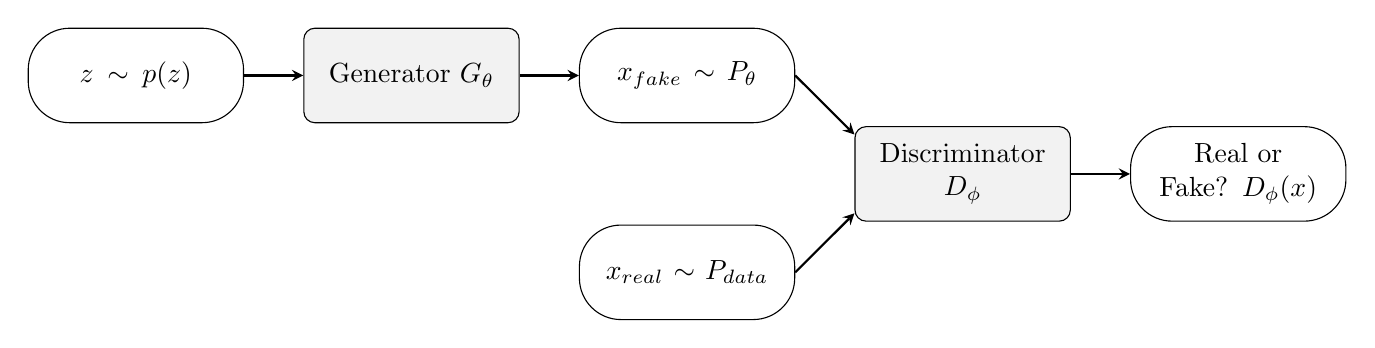
\begin{tikzpicture}[
    box/.style={draw, rectangle, minimum width=2.5cm, minimum height=1.2cm, fill=gray!10, rounded corners, text width=2.5cm, align=center},
    ell/.style={draw, rectangle, rounded corners=15pt, minimum width=2.5cm, minimum height=1.2cm, text width=2.5cm, align=center},
    arr/.style={-stealth, thick}
]
    % Nodes
    \node (z) at (0, 0) [ell] {$z \sim p(z)$};
    \node (G) at (3.5, 0) [box] {Generator $G_\theta$};
    \node (xfake) at (7, 0) [ell] {$x_{\text{fake}} \sim P_\theta$};
    
    \node (xreal) at (7, -2.5) [ell] {$x_{\text{real}} \sim P_{\text{data}}$};
    
    \node (D) at (10.5, -1.25) [box] {Discriminator $D_\phi$};
    
    \node (out) at (14, -1.25) [ell] {Real or Fake? $D_\phi(x)$};
    
    % Arrows
    \draw[arr] (z) -- (G);
    \draw[arr] (G) -- (xfake);
    \draw[arr] (xfake.east) -- (D.160);
    \draw[arr] (xreal.east) -- (D.200);
    \draw[arr] (D) -- (out);
\end{tikzpicture}
\caption{The Generative Adversarial Network architecture. The discriminator $D_\phi$ acts as a learned loss function for the generator $G_\theta$.}
\label{fig:gan_arch}
\end{figure}

\section{Global Optimality and the Jensen-Shannon Divergence}

We first determine the optimal strategy for the discriminator given any fixed generator. Let $p_{\text{data}}(x)$ and $p_\theta(x)$ denote the probability density functions of $P_{\text{data}}$ and $P_\theta$, respectively.

\begin{theorem}[Optimal Discriminator]
\label{thm:optimal_d}
For any fixed generator distribution $P_\theta$ with density $p_\theta(x)$, the optimal discriminator $D^*_\theta(x)$ that maximizes $V(G_\theta, D)$ is given by:
\begin{equation}
    D^*_\theta(x) = \frac{p_{\text{data}}(x)}{p_{\text{data}}(x) + p_\theta(x)}.
\end{equation}
\end{theorem}

\begin{proof}
For a fixed $G_\theta$, the discriminator's objective is to maximize $V(G_\theta, D)$. Writing the expectations as integrals over $\mathcal{X}$, we have:
\begin{align*}
    V(G_\theta, D) &= \int_{\mathcal{X}} p_{\text{data}}(x) \log D(x) \, dx + \int_{\mathcal{X}} p_\theta(x) \log (1 - D(x)) \, dx \\
    &= \int_{\mathcal{X}} \Big[ p_{\text{data}}(x) \log D(x) + p_\theta(x) \log (1 - D(x)) \Big] dx.
\end{align*}
Because $D$ can represent any function, we can maximize the integrand point-wise for every $x \in \mathcal{X}$. Consider a function $f(y) = a \log y + b \log (1 - y)$ for $y \in (0, 1)$ and constants $a, b \ge 0$ (excluding the trivial case $a=b=0$). The derivative with respect to $y$ is:
\begin{equation}
    \frac{df}{dy} = \frac{a}{y} - \frac{b}{1 - y}.
\end{equation}
Setting the derivative to zero yields the maximum at $y^* = \frac{a}{a + b}$. Substituting $a = p_{\text{data}}(x)$ and $b = p_\theta(x)$, the optimal discriminator value for any $x$ is exactly $D^*_\theta(x) = \frac{p_{\text{data}}(x)}{p_{\text{data}}(x) + p_\theta(x)}$. 
\end{proof}

With the optimal discriminator characterized, we can study the generator's objective. By substituting $D^*_\theta$ back into the value function, we expose the underlying divergence metric that GANs implicitly minimize.

\begin{theorem}[Global Optimality of the Generator]
\label{thm:global_g}
The global minimum of the virtual training criterion $C(G_\theta) = \max_{D} V(G_\theta, D)$ is achieved if and only if $P_\theta = P_{\text{data}}$. At this optimal point, $C(G_\theta) = -\log 4$.
\end{theorem}

\begin{proof}
Substitute the optimal discriminator $D^*_\theta(x)$ into $V(G_\theta, D)$:
\begin{align*}
    C(G_\theta) &= \mathbb{E}_{x \sim P_{\text{data}}} \left[ \log \frac{p_{\text{data}}(x)}{p_{\text{data}}(x) + p_\theta(x)} \right] + \mathbb{E}_{x \sim P_\theta} \left[ \log \frac{p_\theta(x)}{p_{\text{data}}(x) + p_\theta(x)} \right].
\end{align*}
To frame this in terms of standard divergences, we multiply the numerator and denominator inside the logarithms by $\frac{1}{2}$:
\begin{align*}
    C(G_\theta) &= \mathbb{E}_{x \sim P_{\text{data}}} \left[ \log \left( \frac{p_{\text{data}}(x)}{\frac{p_{\text{data}}(x) + p_\theta(x)}{2}} \cdot \frac{1}{2} \right) \right] + \mathbb{E}_{x \sim P_\theta} \left[ \log \left( \frac{p_\theta(x)}{\frac{p_{\text{data}}(x) + p_\theta(x)}{2}} \cdot \frac{1}{2} \right) \right] \\
    &= -\log 4 + D_{\text{KL}}\left(P_{\text{data}} \parallel \frac{P_{\text{data}} + P_\theta}{2}\right) + D_{\text{KL}}\left(P_\theta \parallel \frac{P_{\text{data}} + P_\theta}{2}\right).
\end{align*}
This sum of Kullback-Leibler divergences is exactly twice the Jensen-Shannon Divergence ($D_{\text{JSD}}$):
\begin{equation}
    C(G_\theta) = -\log 4 + 2 \cdot D_{\text{JSD}}(P_{\text{data}} \parallel P_\theta).
\end{equation}
Since $D_{\text{JSD}}(P \parallel Q) \ge 0$ for any two distributions and is zero if and only if $P = Q$, the global minimum of $C(G_\theta)$ is $-\log 4$, occurring precisely when $P_\theta = P_{\text{data}}$.
\end{proof}

\section{Vanishing Gradients and the Saturation Regime}

While the minimax formulation guarantees that $P_\theta$ will converge to $P_{\text{data}}$ given optimal discriminators and infinite capacity, practical gradient descent often fails dramatically. To understand why, we must examine the gradients passed from the discriminator to the generator.

The minimax generator loss is defined as:
\begin{equation}
    \mathcal{L}_G(\theta) = \mathbb{E}_{z \sim p(z)} [\log(1 - D_\phi(G_\theta(z)))].
\end{equation}
Let us analyze the gradient of this loss with respect to a generated sample $x = G_\theta(z)$:
\begin{equation}
    \nabla_x \log(1 - D_\phi(x)) = \frac{-1}{1 - D_\phi(x)} \nabla_x D_\phi(x).
\end{equation}

Early in training, the generator's output is poor, meaning $P_\theta$ and $P_{\text{data}}$ are disjoint or highly distinct. Consequently, the discriminator rapidly learns to perfectly separate them, yielding $D_\phi(G_\theta(z)) \approx 0$. As $D_\phi(x) \to 0$, the term $\frac{-1}{1 - D_\phi(x)}$ approaches $-1$. The discriminator function $D_\phi(x)$ becomes extremely flat (due to the saturation of its output sigmoid function) near the generated samples, causing $\nabla_x D_\phi(x) \to 0$. Thus, the generator receives a vanishing gradient exactly when it most needs a strong signal to improve.

To circumvent this, practitioners replace the minimax generator loss with the \textit{nonsaturating} generator loss:
\begin{equation}
    \mathcal{\tilde{L}}_G(\theta) = -\mathbb{E}_{z \sim p(z)} [\log(D_\phi(G_\theta(z)))].
\end{equation}
Here, the gradient with respect to $x$ is:
\begin{equation}
    \nabla_x [-\log D_\phi(x)] = \frac{-1}{D_\phi(x)} \nabla_x D_\phi(x).
\end{equation}
When $D_\phi(x) \to 0$ early in training, the magnitude $\frac{1}{D_\phi(x)} \to \infty$. This amplification counters the flatness of $\nabla_x D_\phi(x)$, providing a massive, non-vanishing gradient signal to the generator.

\begin{figure}[htpb]
\centering
\begin{tikzpicture}[scale=1.2]
    % Axes
    \draw[->, thick] (0, -4.5) -- (0, 2.5) node[above] {Generator Loss};
    \draw[->, thick] (0, 0) -- (5.5, 0) node[right] {$D_\phi(G(z))$};
    
    % Ticks
    \draw (5, 0.1) -- (5, -0.1) node[below] {$1$};
    \node[below left] at (0,0) {$0$};
    
    % Minimax loss: log(1-x)
    \draw[thick, red, dashed, domain=0:4.95, samples=100] plot (\x, {ln(1 - \x/5)});
    
    % Nonsaturating loss: -log(x)
    \draw[thick, blue, domain=0.05:5, samples=100] plot (\x, {-ln(\x/5)});
    
    % Legend
    \node[red, anchor=west] at (2.5, -2) {Minimax: $\log(1-D)$};
    \node[blue, anchor=west] at (1.5, 1.8) {Nonsaturating: $-\log(D)$};
\end{tikzpicture}
\caption{Comparison of generator loss functions. Early in training, the discriminator assigns low probability to fake samples ($D_\phi(G(z)) \approx 0$). The minimax loss (red, dashed) is flat in this regime, yielding vanishing gradients. The nonsaturating loss (blue, solid) exhibits an asymptote at $0$, providing strong initial gradients to propel training.}
\label{fig:gan_loss}
\end{figure}

While the nonsaturating loss resolves the vanishing gradient problem, it changes the theoretical underpinnings of the game. It can be shown that optimizing the nonsaturating loss effectively minimizes a reverse combination of KL divergences. This asymmetric penalty heavily punishes the generation of unrealistic samples but is lenient toward mode dropping, contributing to the empirical phenomenon of \textit{mode collapse} where $P_\theta$ focuses entirely on a small subset of the modes of $P_{\text{data}}$.

\section{Numerical Example: Learning a Gaussian Mean}

To make these pathological gradient mechanics concrete, consider a simple setting where both the true and generated data are one-dimensional Gaussians with unit variance. Let the target distribution be $P_{\text{data}} = \mathcal{N}(\mu^*, 1)$ and the generated distribution be $P_\theta = \mathcal{N}(\theta, 1)$. The generator takes noise $z \sim \mathcal{N}(0, 1)$ and applies the translation $G_\theta(z) = z + \theta$. 

Assuming the discriminator is trained to convergence, we apply Theorem \ref{thm:optimal_d} to find the optimal discriminator:
\begin{equation}
    D^*_\theta(x) = \frac{\exp(-\frac{1}{2}(x - \mu^*)^2)}{\exp(-\frac{1}{2}(x - \mu^*)^2) + \exp(-\frac{1}{2}(x - \theta)^2)}.
\end{equation}
Dividing the numerator and denominator by $\exp(-\frac{1}{2}(x - \mu^*)^2)$, we obtain:
\begin{equation}
    D^*_\theta(x) = \frac{1}{1 + \exp\left( (\mu^* - \theta)x + \frac{1}{2}(\theta^2 - (\mu^*)^2) \right)}.
\end{equation}
This perfectly matches the logistic sigmoid function $D^*_\theta(x) = \sigma(wx + b)$ where the weight is $w = \mu^* - \theta$ and the bias is $b = \frac{1}{2}(\theta^2 - (\mu^*)^2)$.

Let us evaluate the signal received by the generator when it computes the gradient of the standard minimax loss for a generated sample $x = z + \theta$. Note that the derivative of the sample with respect to the parameter is $\frac{\partial x}{\partial \theta} = 1$. By the chain rule, and utilizing the derivative property of the sigmoid function $\sigma'(u) = \sigma(u)(1 - \sigma(u))$:
\begin{align*}
    \nabla_\theta \log(1 - D^*_\theta(G_\theta(z))) &= \frac{-1}{1 - D^*_\theta(x)} \cdot \frac{\partial D^*_\theta(x)}{\partial x} \cdot \frac{\partial x}{\partial \theta} \\
    &= \frac{-1}{1 - D^*_\theta(x)} \Big[ D^*_\theta(x)(1 - D^*_\theta(x)) \cdot w \Big] \cdot 1 \\
    &= -D^*_\theta(x) w \\
    &= D^*_\theta(x) (\theta - \mu^*).
\end{align*}

Consider the regime where the generator is far from the truth, such that $\theta \ll \mu^*$. For a typical fake sample $x \approx \theta$, the discriminator logit evaluated at this sample is:
\begin{equation}
    wx + b = (\mu^* - \theta)\theta + \frac{1}{2}(\theta^2 - (\mu^*)^2) = -\frac{1}{2}(\theta - \mu^*)^2.
\end{equation}
Because the squared distance $(\theta - \mu^*)^2$ is large and positive, the logit is a large negative number, causing the sigmoid output to saturate near zero: $D^*_\theta(x) \approx 0$. 

Consequently, the gradient becomes $\nabla_\theta \log(1 - D^*_\theta) \approx 0 \cdot (\theta - \mu^*) = 0$. The discriminator has perfectly separated the two Gaussians, driving its confidence to 100\% and flattening its decision boundary around the fake samples. Instead of pointing the parameter $\theta$ toward $\mu^*$, the gradient vanishes. This numerically demonstrates the core pathology of the Jensen-Shannon divergence when dealing with disjoint distributions: rather than yielding a gradient proportional to the spatial distance between modes, the gradient decays exponentially, effectively paralyzing the generator.

\begin{horizon}
The fragility of the Jensen-Shannon divergence, illuminated by our Gaussian example, is merely the tip of the topological iceberg. In practice, high-dimensional image distributions $P_{\text{data}}$ and parametrically generated distributions $P_\theta$ are supported on low-dimensional manifolds embedded within a vast ambient space, as posited by the Manifold Hypothesis (Chapter 5). It is conjectured that for any continuous generator mapping, the intersection of these manifolds almost always has measure zero. Thus, a sufficiently powerful discriminator can always achieve perfect separation. Consequently, the true minimax GAN objective is structurally predisposed to gradient starvation in nearly all practical settings.

An open question is whether adversarial training can be mathematically stabilized natively within the standard JSD framework without invoking entirely new distance metrics. While widespread techniques like instance noise, spectral normalization, and gradient penalties artificially enforce Lipschitz continuity on the discriminator---widening its decision boundary to leak signal to the generator---it remains actively debated whether these heuristics secretly optimize alternate mathematical divergences rather than fixing the JSD.

Future work might definitively prove that implicit generative models cannot robustly converge under standard $f$-divergences in high dimensions without exact structural manifold alignment. This limitation strongly motivates the search for metrics that are topologically aware and remain well-defined and differentiable even when supports are disjoint. As we will explore in the upcoming chapters, this realization drives the field's transition from integral probability metrics to optimal transport and Wasserstein distances, fundamentally rewriting the geometric foundations of adversarial learning.
\end{horizon}

\section*{Summary}
\begin{itemize}
    \item Generative Adversarial Networks reframe density estimation as a two-player minimax game, abandoning explicit maximum likelihoods for an implicit generative process $G_\theta(z)$.
    \item Given infinite capacity, the optimal discriminator computes the point-wise ratio of the data density to the combined densities, acting as an adaptive loss function for the generator.
    \item The global optimum of the standard minimax GAN objective occurs when $P_\theta = P_{\text{data}}$, which mathematically corresponds to minimizing the Jensen-Shannon Divergence.
    \item In practice, disjoint distribution supports cause the discriminator to rapidly saturate. This leads to vanishing gradients under the strict minimax loss, forcing the widespread adoption of non-saturating heuristics that alter the convergence dynamics and exacerbate mode collapse.
\end{itemize}

\section*{Exercises}
\begin{enumerate}
    \item \textbf{Optimal Discriminator with Unequal Priors:} Suppose the discriminator is shown real samples with probability $\alpha$ and fake samples with probability $1-\alpha$ (where $\alpha \neq 0.5$). Derive the new optimal discriminator function $D^*_\theta(x)$ that maximizes the modified expected value function.
    \item \textbf{The Nonsaturating Gradient Signal:} Compute the exact gradient $\nabla_\theta [-\log D^*_\theta(G_\theta(z))]$ for the Gaussian example presented in the text. Analyze the behavior of this gradient as $|\theta - \mu^*| \to \infty$. Does it vanish? Prove that it provides a signal pointing toward $\mu^*$.
    \item \textbf{JSD and KL Divergence Bounds:} Prove that $0 \le D_{\text{JSD}}(P \parallel Q) \le \log 2$ for any two probability distributions $P$ and $Q$. Describe the exact conditions under which the upper bound is tight, and connect this to the generator's vanishing gradient problem.
\end{enumerate}

% TODO-CITE: Ensure all named results are cited.
